\newif\ifvimbug
\vimbugfalse

\ifvimbug
\begin{document}

\end{document}
\fi

\exercise{Optimization and Information Theory}
 

\begin{questions}

%----------------------------------------------


\begin{question}{Entropy}{5}
You work for a telecommunication company that uses a system to transmit four different symbols ${S_1, S_2, S_3, S_4}$ through time. 
In the current system, each symbol has a probability to occur according to the following table 
\begin{equation*}
\begin{array}{c|c|c|c|c}
 & S_1 & S_2 & S_3 & S_4 \\
\hline
p_i & 0.03    & 0.62    & 0.26    & 0.09
\end{array}
\end{equation*}
Compute the entropy of the system and write the minimum number of bits requires for transmission.

\begin{answer}
$ H(p) = - \sum_{i=1}^{4}p_i \cdot log_2 p_i = 1.397298 $ \\
Minimum number of bits = $log_2 4$ = 2
\end{answer}

\end{question}

%----------------------------------------------

\begin{question}{Constrained Optimization}{25}
After an upgrade of the system, your boss asks you to change the probabilities of transmission in order to maximize the entropy. However, the new system has the following constraint
\begin{equation*}
    4 = \sum_{i=1}^4 2p_i i.
\end{equation*}
\textbf{1)} Formulate it as a constrained optimization problem. Do you need to include additional constrains beside the one above?
\\
\textbf{2)} Write down the Lagrangian of the problem. Use one Lagrangian multiplier per constraint.
\\
\textbf{3)} Compute the partial derivatives of the Lagrangian above for each multiplier and the objective variable. Is it easy to solve it analytically? 
\\
\textbf{4)} Formulate the dual function of this constrained optimization problem. Solve it analytically.
\\
\textbf{5)} Name one technique for numerically solve these problems and briefly describe it.

\begin{answer}
\textbf{1)}
$ \max\limits_{p} \ J(p) = - \sum\limits_{i=1}^{4}p_i\log_2 p_{i} $\\
s.t.
\begin{math}
\begin{cases}
 f_{1}(p) = \sum\limits_{i=1}^{4} p_{i}i  -2=0 \\f_{2}(p) = \sum\limits_{i=1}^{4} p_{i} -1= 0
\end{cases}
\end{math}\\
\textbf{2)}
\begin{math}
L(p,\lambda) = -\sum\limits_{i=1}^{4} p_{i} \log_2 p_{i}+\lambda_{1}(p_{1}+2p_{2}+3p_{3}+4p_{4}-2)+\lambda_{2}(p_{1}+p_{2}+p_{3}+p_{4}-1) 
\end{math}
\\
\textbf{3)} 
$ \frac{\partial L}{\partial p_{1}} = -\log_2 p_1 - \log_2 e + \lambda_{1} + \lambda_{2} $ \\ \\
$ \frac{\partial L}{\partial p_{2}} = -\log_2 p_2 - \log_2 e + 2 \lambda_{1} + \lambda_{2} $ \\ \\ 
$ \frac{\partial L}{\partial p_{3}} = -\log_2 p_3 - \log_2 e + 3 \lambda_{1} + \lambda_{2} $ \\ \\
$ \frac{\partial L}{\partial p_{4}} =-\log_2 p_4 - \log_2 e + 4 \lambda_{1} + \lambda_{2} $ \\ \\
$ \frac{\partial L}{\partial \lambda_{1}} = p_{1} + 2 p_{2} + 3 p_{3} + 4 p_{4} - 2  $ \\ \\
$ \frac{\partial L}{\partial \lambda_{2}} = p_{1} + p_{2} + p_{3} + p_{4} - 1 $ \\ \\
It is NOT easy to solve it analytically. \\ \\
\textbf{4)} 
Let the derivatives be equal to 0, we are able to write $p_i $ depending on $\lambda_{1}$ and $\lambda_{2}$
$ \frac{\partial L}{\partial p_{1}} = 0 \Rightarrow p_{1}=\frac{1}{e}2^{\lambda_{1}+\lambda_{2}}$ \\ \\
$ \frac{\partial L}{\partial p_{2}} = 0 \Rightarrow p_{2}=\frac{1}{e}2^{2 \lambda_{1}+\lambda_{2}} $ \\ \\ 
$ \frac{\partial L}{\partial p_{3}} = 0 \Rightarrow p_{3}=\frac{1}{e}2^{3 \lambda_{1}+\lambda_{2}}  $ \\ \\
$ \frac{\partial L}{\partial p_{4}} = 0 \Rightarrow p_{4}=\frac{1}{e}2^{4 \lambda_{1}+\lambda_{2}} $ \\ \\
Then: \\
$  L(\theta,\lambda) = - \frac{1}{e}2^{\lambda_{1}+\lambda_{2}} \log_2(\frac{1}{e}2^{\lambda_{1}+\lambda_{2}}) - \frac{1}{e}2^{2 \lambda_{1}+\lambda_{2}} \log_2(\frac{1}{e}2^{2 \lambda_{1}+\lambda_{2}})
- \frac{1}{e}2^{3 \lambda_{1}+\lambda_{2}} \log_2(\frac{1}{e}2^{3 \lambda_{1}+\lambda_{2}}) - \frac{1}{e}2^{4 \lambda_{1}+\lambda_{2}} \log_2(\frac{1}{e}2^{4 \lambda_{1}+\lambda_{2}}) + \\
\lambda_{1} (\frac{1}{e}2^{\lambda_{1}+\lambda_{2}} + \frac{1}{e} 2 \cdot 2^{2 \lambda_{1}+\lambda_{2}} + \frac{1}{e} 3 \cdot 2^{3 \lambda_{1}+\lambda_{2}} + \frac{1}{e} 4 \cdot 2^{4 \lambda_{1}+\lambda_{2}} - 2) 
+ \lambda_{2} (\frac{1}{e}2^{\lambda_{1}+\lambda_{2}} + \frac{1}{e} 2^{2 \lambda_{1}+\lambda_{2}} + \frac{1}{e} 2^{3 \lambda_{1}+\lambda_{2}} + \frac{1}{e} 2^{4 \lambda_{1}+\lambda_{2}} - 1) = \\ \\
= - \frac{1}{e}2^{\lambda_{1}+\lambda_{2}} \left[\log_2 \frac{1}{e} + \lambda_{1} + \lambda_{2} - \lambda_{1} - \lambda_{2} \right] 
- \frac{1}{e}2^{2 \lambda_{1}+\lambda_{2}} \left[\log_2 \frac{1}{e} + 2 \lambda_{1} + \lambda_{2} - 2 \lambda_{1} - \lambda_{2} \right] +\\ \\
- \frac{1}{e}2^{3 \lambda_{1}+\lambda_{2}} \left[\log_2 \frac{1}{e} + 3 \lambda_{1} + \lambda_{2} - 3 \lambda_{1} - \lambda_{2} \right] 
- \frac{1}{e}2^{4 \lambda_{1}+\lambda_{2}} \left[\log_2 \frac{1}{e} + 4 \lambda_{1} + \lambda_{2} - 4 \lambda_{1} - \lambda_{2} \right] -2 \lambda_{1} - \lambda_{2} = \\ \\ \\
= \frac{1}{e} log_2^{e} 2^{\lambda_{2}} \left[2^{\lambda_{1}} + 2^{2 \lambda_{1}} + 2^{3 \lambda_{1}} + 2^{4 \lambda_{1}} \right] - 2 \lambda_{1} - \lambda_{2} \\ \\ $

$ \frac{\partial L}{\partial \lambda_{1}} = \frac{log_2^{e}}{e} 2^{\lambda_{2}} \left[2^{\lambda_{1}} \ln(2) + 2 \cdot 2^{2 \lambda_{1}} \ln(2) + 3 \cdot 2^{3 \lambda_{1}} \ln(2) + 4 \cdot 2^{4 \lambda_{1}} \ln(2)\right] - 2  $ \\ \\
$ \frac{\partial L}{\partial \lambda_{2}} = \frac{log_2^{e}}{e} 2^{\lambda_{2}} \ln(2) \left[2^{\lambda_{1}} + 2^{2 \lambda_{1}} + 2^{3 \lambda_{1}} + 2^{4 \lambda_{1}} \right] - 1  $

Letting the two derivatives be equal to 0, we obtain the following system:
\begin{equation}
\begin{cases}
\frac{1}{e} 2^{\lambda_{2}} \left[2^{\lambda_{1}} + 2 \cdot 2^{2 \lambda_{1}} + 3 \cdot 2^{3 \lambda_{1}} + 4 \cdot 2^{4 \lambda_{1}} \right] = 2\\ 
\frac{1}{e} 2^{\lambda_{2}} \left[2^{\lambda_{1}} + 2^{2 \lambda_{1}} + 2^{3 \lambda_{1}} + 2^{4 \lambda_{1}} \right] = 1
\end{cases}
\end{equation}

Dividing the first equation by the second one and letting $x=2^{\lambda_{1}}$, we obtain: \\ \\
$ \frac{x+2x^{2}+3x^{3}+4x^{4}}{x+x^{2}+x^{3}+x^{4}}=2 \Rightarrow \frac{1+2x+3x^{2}+4x^{3}}{1+x+x^{2}+x^{3}}=2 
\Rightarrow 2x^{3}+x^{2}-1=0 \Rightarrow x \approx 0.6573  \Rightarrow 2^{\lambda_{1}} \approx 0.6573 \Rightarrow \lambda_{1} = -0.6054 $ \\ \\
$ 2^{\lambda_{2}} = e \frac{1}{2^{\lambda_{1}}+ 2^{2 \lambda_{1}} + 2^{3 \lambda_{1}} + 2^{4 \lambda_{1}}} \approx 1.7425 \Rightarrow \lambda_{2} \approx 0.8012 $ \\ \\
$ p_{1}=\frac{1}{e}(0.6573)(1.7425)=0.4213 $ \\ \\
$ p_{2}=\frac{1}{e}(0.6573)^{2}(1.7425)=0.277 $ \\ \\
$ p_{3}=\frac{1}{e}(0.6573)^{3}(1.7425)=0.182 $ \\ \\
$ p_{4}=\frac{1}{e}(0.6573)^{4}(1.7425)=0.12 $ \\

\textbf{5)} We can use the steepest descent method: it is a first-order iterative optimization algorithm for finding a local minimum of a function. It uses  steps that are proportional to the opposite of the gradient of the function at the current point. However if steps are proportional to the gradient, the method returns a local maximum of that function (gradient ascent).
\end{answer}

\end{question}
	

%----------------------------------------------

\begin{question}{Numerical Optimization}{10}
Rosenbrock's function (to be minimized) is defined as 
$$f(\boldsymbol{x}) = \sum_{i=1}^{n-1} \left[ 100 (x_{i+1} - x_{i}^{2})^{2} + (x_{i} - 1)^{2}\right].$$
Write in Python a simple gradient descent algorithm and simulate it for 10,000 steps on Rosenbrock's function with $n=20$. Attach a snippet of your algorithm, discuss the effects of the learning rate and attach a plot of your learning curve with your best learning rate.

\begin{answer}
\lstinputlisting[language=Python]{Rosembrock.py}
\medskip \medskip
The learning rate determines how fast or slow the algorithm will move towards the optimal weights. If the learning rate is very large the algorithm will skip the optimal solution. If it is too small the algorithm will need too many iterations to converge to the best values.
In this case the best learning rate is $ 10^{-6} $. The plot rapresents the parameters curve that tend to the minimum value. \\
\begin{center}
	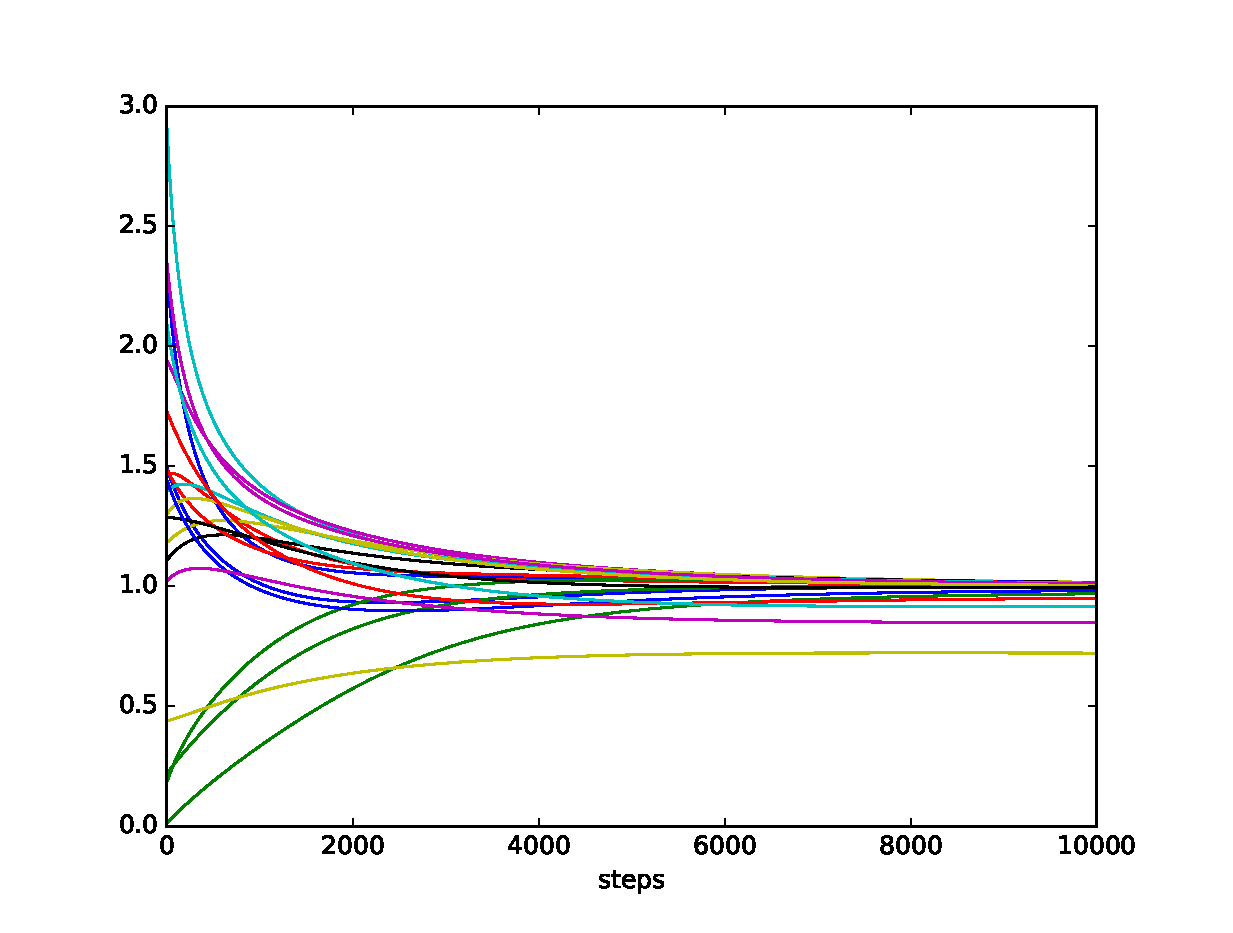
\includegraphics [scale=0.75]{rosembrockPlot.eps}
\end{center}

\end{answer}

\end{question}

%----------------------------------------------

\begin{question}[bonus]{Natural Gradient}{10}
Let $\theta \in \mathbb{R}^n$ be a parameter vector
and $J \colon \mathbb{R}^n \to \mathbb{R}$ a cost function.
The negative gradient $-\nabla J(\theta)$ is sometimes called
the \emph{steepest descent direction}. But is it really?
To be able to claim that it is \emph{the} steepest descent direction,
we should compare it to other descent directions
and pinpoint what is so unique about the negative gradient direction.

\textbf{Covariant gradient.}
A fair way to compare descent directions is to make
a small step of fixed length, say $\varepsilon$,
in every direction~$\Delta \theta$ and check
which direction leads to the greatest decrease in $J(\theta)$.
Since we assume that the step size is small, we can evaluate
the decrease in $J(\theta)$ using its first-order Taylor approximation
\begin{equation*}
  J(\theta + \Delta \theta) - J(\theta) \approx
  \nabla J(\theta)^T \Delta \theta.
\end{equation*}
To make precise what we mean by `small' step size,
we need to introduce a norm (or a distance)
in the space of parameters $\theta$.
A good choice, that among other advantages captures the intuition
that some parameters may influence the objective function more
than others,
is the generic quadratic norm
\begin{equation*}
  \norm{\Delta \theta}^2 =
  \frac{1}{2}\Delta \theta^T F(\theta) \Delta \theta
\end{equation*}
with a positive-definite matrix $F(\theta)$;
note that in general $F$ may depend on $\theta$.

\textbf{1)} Find the direction $\Delta \theta$ that yields
the largest decrease in the linear approximation of $J(\theta)$
for a fixed step size~$\varepsilon$.
Does this direction coincide with $-\nabla J(\theta)$?
The direction that you found is known as the
negative covariant gradient direction.

\textbf{Natural gradient.}
In statistical models, parameter vector $\theta$ often
contains parameters of a probability density function $p(x; \theta)$
(for example, mean and covariance of a Gaussian density);
thus, the cost function $J$ depends on~$\theta$ indirectly
through $p(x; \theta)$.
This two-level structure gives a strong hint as to what matrix $F$
to pick for measuring the distance in the parameter space
in the most `natural' way.
Namely, one can carry over the notion of `distance' between
probability distributions $p(x; \theta + \Delta \theta)$
and $p(x; \theta)$ (which is known from information theory
to be well captured by the Kullback-Leibler divergence)
to the distance between the corresponding parameter vectors
$\theta + \Delta \theta$ and $\theta$.

\textbf{2)} Obtain the quadratic Taylor approximation
of the KL divergence
from $p(x; \theta)$ to $p(x; \theta + \Delta \theta)$ in the form
\begin{equation*}
  KL(p(x; \theta + \Delta \theta) || p(x; \theta)) \approx
  \frac{1}{2}\Delta \theta^T F(\theta) \Delta \theta.
\end{equation*}
Covariant gradient with the matrix $F(\theta)$ that you found
is known as the natural gradient.

\begin{answer}
\textbf{1)} $ \underset{\Delta \theta}{\operatorname{argmin}} \ \nabla J(\theta)^{T}\Delta \theta $ \ \ \ \ s.t. $ \frac{1}{2}\Delta \theta^{T}F(\theta)\Delta \theta=\epsilon^{2} $. \\
Let $ F(\theta)=\epsilon^{2} D^{T}D $ and $ z=D\Delta \theta $ \\ \\
$ \underset{\Delta \theta}{\operatorname{argmin}} \ \Delta \theta^{T} \nabla J(\theta) $ \ \ \ \ s.t. $ z^{T}z=1 $ \\ \\
$ D^{-1} \ \underset{z}{\operatorname{argmin}} (D^{-1}z)^{T}\nabla J(\theta) $ \ \ \ \ s.t. $ z^{T}z=1 $ \\ \\
$ D^{-1} \ \underset{z}{\operatorname{argmin}} \ z^{T}D^{-T}\nabla J(\theta) $ \ \ \ \ s.t. $ z^{T}z=1 $ \\ \\
$ \propto D^{-1}[-D^{-T}\nabla J(\theta)]\propto - F(\theta)^{-1}\nabla J(\theta) $ \\ \\

\textbf{2)} We know that: \\ \\
$ \log \frac{P(x;\theta + \Delta \theta)}{P(x;\theta)} = \log P(x;\theta + \Delta \theta) - \log P(x;\theta) \approx 
\frac{\partial}{\partial \theta} \log P(x;\theta)^{T} \Delta \theta + \frac{1}{2} \Delta \theta^{T} \frac{\partial^{2}}{\partial \theta^{2}} \log  P(x;\theta)\Delta \theta $. \\ \\
Hence: \\
$ D_{KL}(P(x;\theta + \Delta \theta) || P(x;\theta)) = \sum \limits_{x} P(x;\theta + \Delta \theta) \log \frac{P(x;\theta + \Delta \theta)}{P(x;\theta)} $ \\ \\
$ \simeq \sum \limits_{x} [P(x;\theta) + \frac{\partial}{\partial \theta} P(x;\theta)^{T} \Delta \theta + \frac{1}{2}\Delta \theta^{T} \frac{\partial^{2}}{\partial \theta^{2}} P(x;\theta)\Delta \theta] \cdot [\frac{\partial}{\partial \theta} \log P(x;\theta)^{T}\Delta \theta + \frac{1}{2} \Delta \theta^{T} \frac{\partial^{2}}{\partial \theta^{2}} \log P(x;\theta)\Delta \theta] $ \\ \\
$ \simeq \sum \limits_{x} \left[P(x;\theta) (\frac{\frac{\partial}{\partial \theta} P(x;\theta)}{P(x;\theta)})^{T}\Delta \theta + \frac{1}{2}\Delta \theta^{T}P(x;\theta) \cdot
\frac{P(x;\theta) \frac{\partial^{2} P(x;\theta)}{\partial \theta^{2}} - (\frac{\partial P(x;\theta)}{\partial \theta})^{T}(\frac{\partial P(x;\theta)}{\partial \theta})}{P^{2}(x;\theta)} \cdot \Delta \theta \right ] + \\ \\
+ \sum \limits_{x}\Delta \theta^{T} (\frac{\partial}{\partial \theta} P(x;\theta)) (\frac{\frac{\partial}{\partial \theta} P(x;\theta)}{P(x;\theta)})^{T} \Delta \theta $ \\ \\

$ = \sum \limits_{x} \left[ (\frac{\partial}{\partial \theta} P(x;\theta))^{T}\Delta \theta + \frac{1}{2}\Delta \theta^{T}(
 \frac{\partial^{2} P(x;\theta)}{\partial \theta^{2}} -P(x;\theta)(\frac{\frac{\partial P(x;\theta)}{\partial \theta}}{P(x;\theta)})^{T}(\frac{\frac{\partial P(x;\theta)}{\partial \theta}}{P(x;\theta)})) \cdot \Delta \theta \right ]  \\ \\
+ \sum \limits_{x}\Delta \theta^{T} (\frac{\partial}{\partial \theta} P(x;\theta)) (\frac{\frac{\partial}{\partial \theta} P(x;\theta)}{P(x;\theta)})^{T} \Delta \theta $ \\ \\

$ = (\frac{\partial}{\partial \theta} \sum \limits_{x}P(x;\theta))^{T} \Delta \theta + \frac{1}{2} \Delta \theta^{T} (\frac{\partial^{2}}{\partial \theta^{2}}\sum \limits_{x}P(x;\theta)) \Delta \theta + 
\frac{1}{2} \Delta \theta^{T} (\sum \limits_{x} P(x;\theta) (\frac{\partial}{\partial \theta} \log P(x;\theta))(\frac{\partial}{\partial \theta} \log P(x;\theta))^{T})\Delta \theta $ \\ \\ 
$ = (\frac{\partial}{\partial \theta} 1)^{T} \Delta \theta + \frac{1}{2} \Delta \theta^{T} (\frac{\partial^{2}}{\partial \theta^{2}}1) \Delta \theta + 
\frac{1}{2} \Delta \theta^{T} (\sum \limits_{x} P(x;\theta) (\frac{\partial}{\partial \theta} \log P(x;\theta))(\frac{\partial}{\partial \theta} \log P(x;\theta))^{T})\Delta \theta $ \\ \\ 
$ = \frac{1}{2} \Delta \theta^{T}F(\theta)\Delta \theta $
\end{answer}

\end{question}

%----------------------------------------------

\begin{question}[bonus]{Gradient Descent Variants}{5}
Throughout this class we have seen that gradient descent is one of the most used optimization techniques in Machine Learning. This question asks you to deepen the topic by conducting some research by yourself.

\textbf{1)} There are several variants of gradient descent, namely \emph{batch, stochastic} and \emph{mini-batch}. Each variant differs in how much data we use to compute the gradient of the objective function. 
Discuss the differences among them, pointing out pros and cons of each one.

\textbf{2)} Many gradient descent optimization algorithms use the so-called \emph{momentum} to improve convergence. What is it? Is it always useful?

\begin{answer}
\textbf{1)} In Gradient Descent methods, parameters have to be updated according to the following formula: \\ $\theta=\theta + \alpha \nabla J(\theta)$.	\\
Suppose we have data ${(x_i,y_i)}, \\ i=1:M$
\begin{itemize}
	\item Batch GD: All data are used to compute the approzimation of $\nabla J(\theta)$: \\
	$\nabla J(\theta) = \frac{1}{M}\sum \limits _{i=1}^M(\widehat{y_i}-y_i)x_i$
	\item Stochastic GD: Only a sample is used to compute the approzimation of $\nabla J(\theta)$:\\
	$\nabla J(\theta) =(\widehat{y_i}-y_i)x_i$
	\item Mini-batch GD: Only N data are used to compute the approzimation of $\nabla J(\theta)$:\\
	$\nabla J(\theta) = \frac{1}{N}\sum \limits _{i=1}^N(\widehat{y_i}-y_i)x_i$
\end{itemize}
Batch (and Mini-Batch) gradient descent is more computationally efficient than stochastic gradient descent and it has a more stable error gradient. However The more stable error gradient may result in premature convergence of the model to a less optimal set of parameters.\\
\textbf{2)} Momentum takes into account the update $\Delta \theta$ at each iteration, and determines the next update as a linear combination of the gradient and the previous update:\\
$\Delta \theta_{n+1} =\alpha \Delta \theta_n - \beta\nabla J(\theta)$
$\theta_{n+1} = \theta_{n} + \Delta \theta_{n+1}$.
\end{answer}

\end{question}

%----------------------------------------------

\end{questions}
